\documentclass[12pt]{article}

%2. Proposal Margin and Spacing Requirements
%
%The proposal must conform to the following requirements:
%
%a. Use one of the following typefaces identified below:
%
%    Computer Modern family of fonts at a font size of 11 points or larger.
%
%A font size of less than 10 points may be used for mathematical formulas or equations, figures, table or diagram captions and when using a Symbol font to insert Greek letters or special characters. PIs are cautioned, however, that the text must still be readable.
%
%b. No more than six lines of text within a vertical space of one inch.
%
%c. Margins, in all directions, must be at least an inch.
%
%These requirements apply to all uploaded sections of a proposal, including supplementary documentation.

%\pagestyle{headings}
\usepackage{sidecap}
\usepackage{setspace}
\singlespacing
\usepackage{url}
\usepackage{hyperref}
\usepackage{graphicx}
\usepackage{amsfonts}
\usepackage{amsmath}
\usepackage{color}
\usepackage{amsbsy}
\usepackage{amssymb}% Include extra symbols: \gtrsim and \lesssim
\usepackage{fancyhdr}
\usepackage{shading}
\usepackage{wrapfig}
\usepackage{xspace}
\bibliographystyle{aasjournal}
%\usepackage{mathpazo,bm}
\usepackage{mathpazo}
\usepackage{natbib}
\usepackage{deluxetable}
\usepackage{mdwlist}
\usepackage{url}
\usepackage{longtable}
\usepackage{rotating}
\usepackage{multicol,multirow}
\usepackage[normalem]{ulem}
%\usepackage{bibtex}
%\usepackage{mathabx}
\usepackage{esint}
\addtolength{\oddsidemargin}{-0.75in}
\addtolength{\evensidemargin}{-0.75in}
\addtolength{\textwidth}{1.55in}
\addtolength{\topmargin}{-0.75in}
\addtolength{\textheight}{1.6in}

\newlength{\hfwidth}
\newlength{\hfwidthsingle}
\addtolength{\hfwidthsingle}{.5\textwidth} %single fig in figure
\addtolength{\hfwidth}{.497\textwidth} %single fig in figure*

%avoid figures from occupying the whole page
\renewcommand{\topfraction}{0.95}
\renewcommand{\textfraction}{0.05}
\renewcommand{\floatpagefraction}{0.85}
\newcommand{\msun}{M$_{\odot}$}
\newcommand{\resitem}[1]{\item #1 \vspace{-2pt}}
%\newcommand{\note}[1]{[$\triangleright\triangleright$~\textbf{#1}~$\triangleleft\triangleleft$]}
\newcommand{\resheading}[1]{{\flushleft{\parashade[.8]{sharpcorners}{\textbf{#1 \vphantom{p\^{E}}}}}}}
\newcommand{\ressubheading}[4]{
\begin{tabular*}{6.5in}{l@{\extracolsep{\fill}}r}
  \textbf{#1} & #2 \\
  \textit{#3} & \textit{#4} \\
\end{tabular*}\vspace{-6pt}}
\newcommand{\shadebox}[1]{\textshade[grayscale]{sharpcorners}}
\newcommand\new[1]{{\color{blue}#1}}
\newcommand\reword[1]{{\color{red}#1}}

\def\apj{\rm ApJ}
\def\apjl{\rm ApJL}
\def\apjs{\rm ApJS}
\def\aj{\rm AJ}
\def\mnras{\rm MNRAS}
\def\araa{\rm ARAA}
\def\nat{\rm Nature}
\def\pasj{\rm PASJ}
\def\pasp{\rm PASP}
\def\aap{\rm A\&A}

\usepackage{geometry}
\geometry{margin=1in}

\makeatletter
\def\@to{to}
\makeatother

\thispagestyle{empty}
\begin{document}


\section{PASSAGE: Project Objectives and Plans}
%%% NSF Text:  %%%
% The project should have specific objectives that reflect the goals of the S-STEM program and local needs, as well as specific plans to select students, encourage them to achieve their best academic performance, and enable them to enter the workforce or continue studies in their fields. The project also should have specific plans to implement and investigate existing high quality evidence-based practices and professional and workforce development activities (e.g., academic and student support activities) and to contribute to the knowledge base about what works for whom in college retention, student success, and graduation (to include transfer, if appropriate) in STEM.

%\noindent
%{\bf Overview}\\
Students from traditionally underrepresented backgrounds often struggle when transitioning from one academic environment to the next.  According to a report published by the National Academies in 2016, the concept of a concrete pipeline for students interested in science, technology, engineering and mathematics (STEM) fields is no longer a accurate metaphor.  Most of these students do not take a straight line on their journey through they education system toward a STEM degree.  A larger percentage of STEM students begin their careers at two year institutions before transferring to a four year institution.  There is also a growing number of students who transfer from four year schools to two year schools, or students who are enrolled in multiple colleges or universities at a time. Increasing the number of these transitions  therefore increases the complications that go along with them. 

In addition, the background, age, goals and preparedness of the students entering the higher education system is becoming more diverse. Students often have a wide variety of responsibilities outside of school that can impact their focus and time commitment to their studies including raising children, caring for older parents, or work commitments.  With an ever increasing number of students indicating an interest in STEM fields, only one half the students planning a STEM bachelor's degree and one third of students attempting a STEM associate's degree succeed in earning those degrees within 6 or 4 years respectively.  These statistics are even more dire when applied to underrepresented groups \citep{NAP21739}. %They often do not follow a  ``traditional'' pathway from high school $\rightarrow$ college $\rightarrow$ graduate school, but take a more circuitous route.  

As a result of these challenges, retaining such students in STEM fields is challenging.
%re-entering school after time off, or dealing with additional circumstances that affect their time commitment and focus. 
This proposal specifically targets these transitions for CUNY community college students (the majority of whom fit within at least one underrepresented demographic) with structures specifically tailored to support and retain them.
{\bf We will implement a community college physics pathway to aid those working toward four-year schools and beyond.} We call our program {\bf PASSAGE} - {\bf P}hysics, {\bf A}stronomy and {\bf S}TEM {\bf S}uccess through {\bf A}ctive and {\bf G}enuine {\bf E}ngagement.  Students will participate in mentoring, advising, community involvement, and research experiences.  Our program will focus on Physics and Astronomy students, which are often linked within the same department.  % and were chosen for several reasons.  
Physics is a broad field where students can apply their interests both in and out of STEM disciplines to exciting topics and research. Astronomy inspires students and the awe and excitement of studying the universe is still strong for many college students.  Physics is an excellent foundation for students in STEM fields because of its broad impact on so many different applications. It is an excellent platform to introduce technical skills, improve critical thinking and problem solving skills.  In addition, physics still lags nationally behind many other STEM fields in terms of participation from minorities and women.  (insert some statistics about that here?)

Students participating in PASSAGE can be expected to experience higher rates of retention and success. %as they traverse the academic maze.  
{\bf Our objective is for  75\% of participating students to achieve a further degree (B.S. or B.A.) in a STEM field, with 50\%  in physics and/or  astronomy.} % Important to say where the numbers come from.  (based on Fisk-Vanderbilt success, I expect blah blah).  
%\vspace{-2mm}
The retention of students in STEM fields has been a challenge.  69\% of community college students who enter STEM fields leave them, either by changing majors or dropping out of college altogether \citep{NCES}.  While Black and Hispanic students are well represented in STEM college major choices, many of these students do not graduate with STEM degrees \citep{Ma15}.  The problem persists at higher levels of education as well; the fraction of science PhDs awarded to African American, Latino, and other minority students is far smaller than the fraction these minorities constitute in the general population \citep{NSF06,Ivie18}.   Similarly, gender imbalances also exist in most science fields: women are underrepresented at the graduate student and faculty levels \citep{NSF04,Ivie18}, and continue to be lost at every educational transition \citep{NAP}. 	Transitions are particularly difficult for marginalized students, who may deal with racism, sexism, ableism, income disparities, and other discriminatory challenges in addition to academic ones.  {\em In this proposal we target the key transition point of community college to four-year university with the aim of increasing the retention and success of marginalized students in physics, astronomy, and other STEM fields.   }


%Underrepresented minority (URM) students and women of all backgrounds drop out of STEM fields at a higher rate than their male/majority peers.   (no ref for this)


%[Community college STEM stats go here, find some to justify my argument]    \\
% 69\% of CC students who enter STEM fields leave them, either by changing majors or dropping out of college altogether.  (dept of education statistical analysis report NCES 2014-001)

%Prior literature indicates that URM students seem to benefit most from intervention 
%programs that promote academic confidence, like undergraduate research programs, because 
%their experiences within math and science course can lead them to doubt their academic ability in 
%these subjects (Perna et al., 2009) and their decisions to remain in a STEM major (Crisp et al, 
%2009).   (from Herrera & Hurtado)

%\vspace{-4mm}

% this paragraph is good but change for physics % I added some words about this earlier Should we keep this in here?
%The field of astronomy (oops, and physics! reword)is an ideal gateway to STEM success.  Students (and the public) are attracted to astronomy because of its ability to inspire and amaze.  In addition to inspiration, however, engaging in astronomy research provides students with many tools, such as data analysis and visualization, software engineering, computation, statistics, and technical communication.  Thus, students with a background in astronomy research are equipped to segue into a plethora of related STEM fields.
	
{\bf The objective of this proposal is to increase the number of traditionally underrepresented people in STEM fields by providing opportunities and support in research, community, and mentorship.} Mentoring relationships are essential to students who continue in STEM fields past their first year \citep{reureport,Nagda,Wilson}, and research experiences are particularly effective in giving underrepresented students the confidence and enthusiasm for taking advanced courses and learning difficult material \citep{armstrong03}. It is our prediction that the same techniques that help retain STEM students past the initial year will also help at critical transition points for students. These initiatives will implement many of the best practices for retaining underrepresented students:  building a sense of community; providing advising, mentoring, and academic support; and engaging students in discipline--specific research \citep{jordan,holland}. 	

\section{Significance of Project}
% %%% NSF Text:  %%%
% A proposal must state and justify with institutional data the annual and total number of unique students who will be awarded scholarships over the duration of the award period, the number of scholarships awarded annually, the total number of scholarships awarded for the award period, the duration of the scholarship, and the annual and maximum amount of the scholarship for a scholarship recipient.

%The proposal should address how the goals of the S-STEM program will be met (see Program Description, Section II). In addition, if appropriate, it should include information on the demographics of the departments or programs affected by the scholarships, including number of majors and number of graduates per year, as well as information on overall enrollment and retention within the institution and programs involved.

%A rationale for the number of scholarships and the scholarship amount requested should also be provided. Specifically, baseline data from Institutional Research Offices should include (1) current student demographics and enrollment from institutions awarding scholarships; (2) current student demographics and enrollment for each S-STEM eligible discipline that is included in the proposed project and the projected number of low-income students that meet the eligibility requirements in those disciplines; (3) current 1-year retention rates for each S-STEM eligible discipline that is included in the proposal; and (4) current graduation rates for each S-STEM eligible discipline that is included in the proposal. This baseline data will also be useful for project evaluation. It may be helpful to consult with the financial aid office at the institution to determine typical financial need for the proposed cohort of students (or for some larger group of students if information on the smaller cohort is not easily available). While there is flexibility within a project budget after a grant is made, the size of the budget request must be closely related in the proposal to a realistic estimate of student need.

%For S-STEM eligible disciplines included in the proposal, expected outcomes should include, at a minimum: expected demographics and enrollment for the disciplines that are included in the proposal showing the current number of low-income students that would qualify for the scholarships; expected year to year retention or transfer rates for S-STEM eligible disciplines for the eligible student population that are included in the proposal; expected graduation rates for each of the S-STEM disciplines included in the proposal and/or expected student outcomes documenting students successfully overcoming one or more of an institution’s self-identified attrition points.
	
Community colleges often host large numbers of minority students, and Queensborough Community College (QCC) is no exception.  Out of the 14,000 enrolled QCC students, 29\% are Hispanic/Latinx, 28\% are Asian, 28\% are African American, and 14\% are Caucasian.  34\% of QCC students speak a language other than English at home, and over 50\% come from a family with an income below \$25,000 per year \citep{QCCweb}. The QCC student body is an ideal pool of students to target for PASSAGE.


The declared STEM majors at QCC exhibit similar demographics to the overall student body, but with a higher fraction of Asian students and a lower fraction of Hispanic and Black students.  44\% of QCC students are identified as low-income, based on receipt of Pell grants, and this fraction is unchanged for STEM majors.  While one-year retention rates are somewhat high (62\% for all students, 74\% for STEM majors), three-year graduation rates at QCC are extremely poor; in the past few years, the rate has ranged from 22-28\% for all students and 10-30\% for STEM majors (data compiled by the QCC Office of Institutional Research and Assessment, 4/10/2020).  There is clearly a leak in this pipeline -- many students wish to major in STEM but few succeed in acquiring a major in a timely fashion.  We seek to increase these abysmal numbers by putting support structures into place which will retain QCC students, and specifically those from underrepresented backgrounds.


%  QCC info:  http://www.qcc.cuny.edu/about/fast-facts.html
% more than 50% of students come from a family with income below $25,000 
% from 127 nations speaking 78 native languages
%  25% AfAm, 30% hispanic, 29% asian, 15% caucasian
%  more than 20% are immigrants, and 34% speak not-English at home

QCC students are not well-informed about the career opportunities and skills a physics major can provide.  
Those interested in technical fields often gravitate towards engineering, due to the seemingly straightforward career path and high earning capabilities.  The students who {\em do} follow a physics major trajectory often receive erroneous advice on course registration, resulting in the unnecessary repetition of coursework.  These students often stumble as they traverse the academic maze, unless they are fortunate enough to find a faculty mentor who can guide them.  PASSAGE will recruit low-income, underrepresented students into the physics major; provide them with mentoring, community, and financial support; and prepare them to succeed on the path toward their bachelor's degree.




\section{Current Activities in the Physics Department}
%%% NSF Text: %%%
% S-STEM projects should build on the research literature and existing academic and student supports and program elements. Proposals should discuss such academic and student supports and program elements that are relevant to the S-STEM project and describe ways in which the S-STEM project will use or enhance the structures. Proposals should describe and justify the adaptation of academic and student supports and program elements implemented for S-STEM Scholars and other STEM students. If the institution or a member of a consortium of institutions has had a previous S-STEM and/or STEP award, show how the proposed project will build on lessons learned from these efforts.

%S-STEM projects should draw on the research literature and discuss the issues or gaps in the literature that the project plans to address.

%\section{Quality Educational Programs}
%  Institutions should provide evidence of the quality of their educational programs, particularly those in the targeted disciplines. Where appropriate, cite external accreditations in the S-STEM disciplines (for example, ABET for engineering).
Queensborough community college is a two year school offering more than 45 different programs of study.  We maintain a middle states accreditation that was renewed in 2019.  The physics department heavily supports a variety of programs such as the engineering science program (A.S), the liberal arts and science program (A.S.), the Science for Forensic program (Dual/Joint).  We are also in the process of creating an associates degree in physics.  In order to provide quality experiences in our physics classes the physics department is very active in Physics education research employing multiple research proven techniques in the classroom including think-pair-share, flipped classrooms, problem based learning and peer instruction. As a department, we also have a rigorous assessment protocol for tracking the effectiveness of these techniques.
\subsection{Research Experience}
Several students are currently undergoing research projects in our department.  Research experiences have been shown to increase the retention of underrepresented minority students in STEM fields \citep{Graham,Russell}.   Such experiences  enable students to gain skills and network, and aid them as they continue their studies.  Several QCC Physics faculty have active research groups (e.g., professors Armendariz, Damas, Dehipawala, Marchese, Riegel, Taibu and Bellovary), and all faculty are encouraged to engage students in research projects.  Our department hosts and NSF REU program during the summer (focusing on students from nearby community colleges who have no access to research) and also engages QCC students all year round.  S-STEM scholars will be mentored by QCC Physics faculty in research during the school year and during their first summer summer of the program.  During the summer, faculty mentors will receive \$2950 in summer salary for each S-STEM scholar they mentor.  In exchange, faculty will provide regular guidance and check-ins, assess student development using a modified IDP form (see Section \ref{sect:IDP}), and report to the program directors Bellovary and Riegel regularly about student progress.  
%\new{more?  Not sure, should they be involved in the IDP updating?  I don't want to require too many things from people because they are lazy and just won't do it. But sometimes providing structure is good so, I'm torn.  Perhaps a semester report form, not more than a page or a semester update of the IDP?}

This proposal builds on the strong research foundation of our department and incorporates the supported students within the current research infrastructure.  With so many faculty engaging students, there will be a plethora of projects available for students in the program, with a range of physics subfields.  All students who engage in research must undergo the Responsible Conduct in Research online and in-person training, and our S-STEM scholars will do this as well.

\subsection{Preparing for Research: Physics 450}
Students prepare for research projects by taking the Physics 450 course ``Introduction to Physics Research'' during their first year in the program.   Topics for this course include scientific reading and writing, keeping a lab notebook, designing an experiment, writing a literature review, analyzing data, basic data visualization, and presentation skills.  Faculty looking for students in the following semester will give presentations during the class to recruit students and keep the students informed about the kind of research being performed on the Queensborough campus.  The course instructor will then facilitate matching students with mentors.  The instructor for this course will be sure to emphasize and recruit for the program for students not already enrolled during this course.  In the second half of this course, students will work on individual or group research projects with the goal of writing a literature review and attempting basic data analysis.  For example, a student could use python to measure the density profile of a simulated dwarf galaxy, and determine whether it has a cusp or a core.  By the end of the course, students will have the rudimentary skills to leap into research.  

\subsection{Associates of Science in Physics}
At the time of writing this proposal, the physics department has developed the curriculum for an Associates degree in Physics (A.S.).  The program is currently undergoing the required approvals process for the University.  Having a formalized program with clear prerequisites, course requirements, and transfer expectations will greatly facilitate the creation of a pipeline of physics majors.  Students will receive improved and streamlined advising in this program, compared to the hodgepodge they receive today.  

One course we are adding to the physics major program is the ``Colloquium Course,'' which involves a weekly seminar on a current topic in physics.  This seminar will excite students as well as build cohesion among the physics majors.  It is also a way to engage physics majors in the department and give them an opportunity to engage with faculty before they have completed the introductory course.  This interaction with the physics department is particularly important for students who lack the math skills to take the other required physics classes in their first semester to ensure that they feel welcomed and engaged with the physics department.

\section{New Activities in the Physics Department}

This proposal aims to create a financially-supported, tightly knit cohort of physics majors who are ready to succeed as they transfer to a four-year college.  We will continue our current practice of engaging students in research, but in addition we will  create a comprehensive, formalized trajectory for physics majors at QCC, including:
\vspace{-2mm}

% make the order more logical
% consider reducing to categories and making sub-points (to make it seem less ambitious)
\begin{itemize}
\setlength{\itemsep}{-\parsep}
\setlength{\topsep}{-\parsep}
\setlength{\partopsep}{-\parsep}
	\item connect students to research opportunities within the QCC Physics department \& elsewhere (currently happening)
	\item design and implement an Associate's Degree (A.S.) in Physics (in progress)
	\item design brochures for advisors and professors to hand out to interested students
	\item create a portion of the department website dedicated to physics major requirements, activities and opportunities
	\item facilitate seminars and panels on career options, networking, applying to internships, etc.
	\item build a sense of community among physics majors 
	\item offer financial support 	
\end{itemize}	
	
To recruit and retain students, we will create brochures and flyers which will advertise our PASSAGE program.  Students as well as academic advisors and professors in other departments must become familiar with it in order for it to succeed.  These brochures will contain the information described above, highlighting the preparedness for transferring and the eventual job prospects of those who major in physics and STEM fields. 

Our department website lacks resources for students seeking information on a physics major.  We will redesign portions of it, and add a page specifically aimed at students who want to learn more about the physics major.  This page will link to a description of our program, show examples of research projects that have been done, and contain photos of our students doing research and presenting at conferences.
	
We will create a monthly seminar series for physics majors to promote student success and build community.  This series will include relevant topics such as applying for internships, getting research experience, and writing a CV.  QCC students lack this guidance, and a solidified communication channel will greatly increase their success.

A sense of community is vital in retaining underrepresented students in STEM \citep[][and references therein]{NAP25257}.  A sense of belonging to a community increases confidence and improves success rates.   and We will foster cohort-building within each year's intake and across cohorts by planning monthly social events as well as annual field trips to nearby locations of interest.  Experiencing STEM-relevant activities with a larger group of students and faculty acknowledges a shared interest, reinforces positive attitudes toward STEM, and grows family-like ties among participants.  In Section \ref{sect:IDP} we further discuss mentoring and support structures which foster community.

Lastly, to aid our students in focusing on their difficult coursework without distractions, we will support them financially with scholarships, according to each students' financial need.  This support will release our students from the need of part-time jobs which take time away from academic activities.  The scholarships are described in detail in Section \ref{sect:money}.



\section{S-STEM Project Management Plan}\label{sect:money}
%%% NSF Text  %%
% S-STEM projects must be guided by a management plan in which the key personnel and project logistics are defined. The roles and responsibilities of the personnel involved should be clear.

%For all projects the project leadership team must include a faculty member currently teaching in an S-STEM eligible discipline as listed in Section IV.B, a STEM administrator, and an institutional, educational, or social science researcher.

%The project must involve S-STEM faculty, as mentors, in addition to the PI, and it is strongly encouraged that the project involve staff from offices of institutional research, student services, financial aid, and/or admissions. These additional personnel may be included as Co-PIs, depending on institutional policy. In any case, the proposal must describe specific roles of each person in the project. The PI will have overall responsibility for administering the project and for interacting with NSF.

%Plans must be described for activities such as recruitment, selection, and retention of students; studies to determine the effectiveness of project activities; maintenance of S-STEM records; coordination of data collection, analysis, and reporting responsibilities; oversight of student supports; and implementation of a process by which students who lose S-STEM eligibility will be replaced by new students.

Financial support is critical for community college students, who are often low-income and working at least one job in addition to taking classes.  Giving students the freedom to focus on coursework is the best support we can give.  We propose to offer several scholarships per year to qualified students who engage in research projects within our groups.  In order to roll out the program in a manageable way, we will increase the number of student recipients each year.  In year 1 we will begin with 4 students, followed by 6 in year 2, 8 in year 3, and 10 in year 4, for a total of 28 students.  In year 5 we will focus on mentoring our existing cohorts, though we may evaluate our remaining funds and admit some new students as we are able.

Student scholarships will be managed by the QCC Office of Grants and Sponsored Programs (OGSP), following standard CUNY procedures (see Budget Justification for more details).  Scholarships will be based on need as calculated by the QCC Office of Financial Services (OFS), which is done for every student at QCC who receives financial aid.  The OGSP regularly coordinates with the OFS for scholarships of this type.  


To maximize retention of the participating students after they leave QCC, we will continue their financial support for two subsequent years, presuming they transfer to a 4-year institution and continue to pursue a physics or astronomy major.  Regardless of the transfer institution, we will establish a relationship with a local mentor to facilitate tracking each students' progress.  This local mentor will aid with advising and course selection, as well as complete a check-in phone call with me at the beginning and end of each semester.  We expect the majority of our students to transfer to a 4-year college within the CUNY system, consistent with current trends.  Within CUNY, there is an existing network of astronomers known as CUNYAstro\footnote{https://cunyastro.org/}, who are located at the majority of CUNY 4-year institutions; thus, transfers to other CUNY physics departments will be absorbed into the existing network of CUNYAstro  mentors.  We will manage the matriculated students by requesting transcripts at the beginning and end of each term to verify their majors and good standing.  We will also check in with each student via phone or Skype each semester to maintain our mentoring relationship, discuss their progress, and consider future opportunities.  Based on the advisor report, transcripts, and check-in, we will authorize continuation of the student scholarship through the next semester.  

QCC students participating in PASSAGE will receive a scholarship as they undergo their research training. Students will be supported with scholarships for 2 years at QCC.  They will also be expected to do research with a faculty mentor during one summer at QCC, for which they will receive a \$5000 stipend.  They will then receive a scholarship for two subsequent years at the four-year institute they transfer to (or until the grant ends, whichever comes first).  Students will be supported for a maximum of four years, regardless of which year they transfer or their graduation status at the end of that time. Student support will only be awarded for full-time students who remain in a physics, astronomy, or other STEM field.  

The maximum scholarship award per year will be \$7,250.  Tuition costs for the 2019-2020 school year are \$4800 per year, and with required fees the total comes to \$5210 per year.  Tuition at 4-year CUNY colleges tuition costs average around \$7,200 per year.  While at minimum our students must cover the cost of tuition, we acknowledge that low-income QCC students qualify for financial aid, and many of them do not pay any tuition.  They must still cover costs such as housing, meals, health care, transportation, etc., and thus the amount of money they receive will be based on their ``need'' as calculated by the OFS.   The maximally allowed value by S-STEM of \$10,000 is unlikely to be required by any of our students, based on their estimated costs, and so we have set the scholarship value lower in order to serve more students.

In summary, the management team consists of the following roles:
\begin{itemize}
\setlength{\itemsep}{-\parsep}
\setlength{\topsep}{-\parsep}
\setlength{\partopsep}{-\parsep}
	\item Office of Grants and Sponsored Programs manages scholarships, tracks eligibility, and requests transcripts from post-QCC students
	\item Office of Financial Services determines eligibility and communicates to OGSP
	\item QCC Physics professors mentor students in research and give general guidance
	\item PI Bellovary and Co-I Riegel find local mentors to post-QCC students and undergo semesterly check-ins
	\item Physics professors who serve as local mentors at transfer institutions, identified by Bellovary and Riegel to communicate student progress
	\item more?
\end{itemize}	


In order to facilitate the program and keep it running smoothly, we request funding for faculty course release, corresponding to 7.1\% effort per year \reword{Christine, how is this worded?}, totalling \$7000? per year.  Community college professors have a heavy teaching load, and having time to focus on the management of the program will be critical in its success.

%\reword{below paragraphs should go back to budget justification, they are so boring.}
%QCC has implemented procedures to ensure that a student who participates in a stipend/fellowship program meets all eligibility requirements of the grant.  No student can be accepted to participate in a grant-funded stipend/fellowship program until OGSP has reviewed his or her application to confirm that he or she meets all the requirements of the grant.  OGSP will collect and maintain on file from the PI the students' transcript, advisor report, and forms required by the Research Foundation of CUNY to process the stipend.  Depending on grant requirements, these may include the QCC Student Eligibility Criteria Form, RFCUNY Data Collection Form, RFCUNY Direct Deposit Authorization form, QCC Student Release of Financial Aid Information.  
 
%Once processed through OGSP and RFCUNY, fellowship payments will be mailed directly from the RFCUNY to the students.  The PI will agree on a payment schedule with the student which will be described in the fellowship award letter which both parties will sign.  The letter from the PI will outline expectations of the student, fellowship requirements, and the period of time covered by the fellowship. 



\section{Student Selection Process and Criteria}
We will select students via an application process which includes a questionnaire, and interview, and a reference contact.  The questionnaire will provide basic information and include financial information with which to determine each students ``need.''  We will coordinate with the financial aid office to verify each candidate's eligibility for S-STEM.  The questionnaire will also ask questions such as ``what are your plans for the future?'' and ``why are you interested in physics?''  During the interview, we will probe more deeply into the answers to these questions.  Lastly, the reference will be contacted to verify the students' good academic standing, motivation, communication skills, and work ethic.

We choose not to use grades or test scores as criteria.  Our target demographic is students entering QCC in their first year, so they may not have college grades available yet.  Such students are often at a turning point in their lives, or may have taken time off before entering QCC, and high school grades are variable and not necessarily relevant.  Standardized test scores are also found to be unrepresentative of a students' true academic potential.

The students targeted in our program will mainly be from underrepresented backgrounds, because we are selecting students from the diverse QCC  student population.  We will also select for those who show ``grit'' and the ability to persevere through challenges.  

An adequate mathematics background is a requirement for any student beginning a physics major.  While we will not examine grades of prior math classes, Calculus I is a co-requisite for our Calculus-based Physics 1 course.  Candidates must demonstrate that they are ready to enter at least pre-Calculus by the time they enter our program, in order to finish the required math courses in a realistic amount of time.


% The program requires that the students meet the requirements for citizenship, discipline, academic potential, and need that are outlined in Section IV.B, Additional Eligibility Information, Scholarship Recipients. Projects should have additional selection criteria that reflect the local program. S-STEM scholarship recipients must be able to demonstrate their eligibility in each semester or quarter of S-STEM support.

%The selection process for scholarship recipients should include indicators of academic merit and other indicators of likely professional success. Multiple indicators may be appropriate in gauging both academic merit (e.g., grade point average, placement test results) and professionalism (e.g., motivation, ability to manage time and resources, communication skills).

%Selection criteria must be flexible enough to accommodate applicants who come from diverse backgrounds (e.g., geographic and with diverse career goals). The program encourages projects to recruit a diverse applicant pool that is inclusive of, but not limited to, members of underrepresented groups in STEM (e.g., females, African Americans, Hispanic Americans, Native Americans, including Alaska Natives and Native Pacific Islanders, persons with disabilities, first generation, rural, veterans), with the broad aim of supporting low-income academically talented students with demonstrated financial need to obtain degrees and enter into the STEM workforce or graduate studies.

%The proposal should indicate how students' eligibility will be determined, the mechanisms by which scholarships for students will be provided, and how scholarship program outcomes will be evaluated and disseminated. It should also identify criteria for retention of students' scholarships from one year to the next.
%These students will be selected by an application process, and will be evaluated on a combination of academic merit and ability to persevere through challenging obstacles.  We will interview potential students and develop a rubric to select and evaluate them.  


\section{Mentoring and Support Structures}\label{sect:IDP}
%  It is expected that awardee institutions will have or will adapt existing high-quality evidence-based practices (e.g., curricular and co-curricular activities; professional, and workforce development activities) designed to enhance student learning, academic performance, retention to graduation, and career or higher education placement. Awardee institutions will implement and test these practices to understand if they are working as expected, if they are successful, and for what types of students.

%Experience indicates that the most successful S-STEM projects involve faculty mentoring and a group of students who in some way naturally associate, whether as majors in the same department, or sharing classes, or participating together in activities of common interest. Thus, in this model, two of the program requirements are that all S-STEM scholarship recipients have STEM faculty mentors and are placed in student cohorts. Other examples of student support activities to consider include:

%    Recruitment of students to higher education programs and careers in the S-STEM eligible disciplines;
 %   Curricular activities such as the inclusion of active learning in gateway courses;
 %   Support and mentoring of students by peers and other professionals;
 %   Academic support services such as tutoring, study-groups, or supplemental instruction programs;
 %   Industry experiences, internship opportunities, and research opportunities;
  %  Community building and support among S-STEM scholars within the institution;
%    Participation in local or regional professional, industrial or scientific meetings and conferences; and
 %   Career counseling and job placement services for S-STEM scholarship recipients.

%For support services and programs that already exist, describe how they will be adapted to meet the specific objectives of the S-STEM project. Partnerships with industry are encouraged.
S-STEM students will receive support from several sources.  PI Bellovary and Co-PI Riegel will interact with all students frequently, especially those at QCC, because they will be overseeing the program, planning social activities, and tracking student progress.  Each student will also have a research mentor, who will be tasked with the professional and skills development of their mentees.  When students transfer to a 4-year college, they will acquire and additional faculty mentor at their new institution.  Students will also be set up with peer mentors in the program.  Lastly, community activities will \new{also be good.}

\subsection{Mentoring by Faculty}

In order to ensure effective mentoring and building a sense of community for the students, we will include a comprehensive mentoring plan to aid students in their physics journey.  The Individual Development Plan (IDP) is a popular tool for graduate students and postdoctoral researchers to help them plan for the next steps in their careers. We propose to apply this for undergraduate physics and astronomy students.  It will provide some scaffolding for the students to plan their trajectory as they navigate some of the crucial transitions throughout their academic career.  It will be important to stress to the undergraduate students that these documents are fluid and changeable so they will be revisited every few months to reevaluate goals and skills.  The IDP will consist of two key components.  The first is a goals assessment which will look at long term, intermediate, short-term, and immediate goals. This will include a timeline, skills required and strategies to get there. The second component will be a skills assessment.  This will help the students determine what academic, research and professional skills they will need and some specific strategies to help acquire these skills. This will help the students figure out what classes they need to take and what programming they should be attending. Sample worksheets for the IDP are provided in the supplemental materials \citep{Bosch}.  \new{provide the thing!}

\begin{figure}
    \centering
    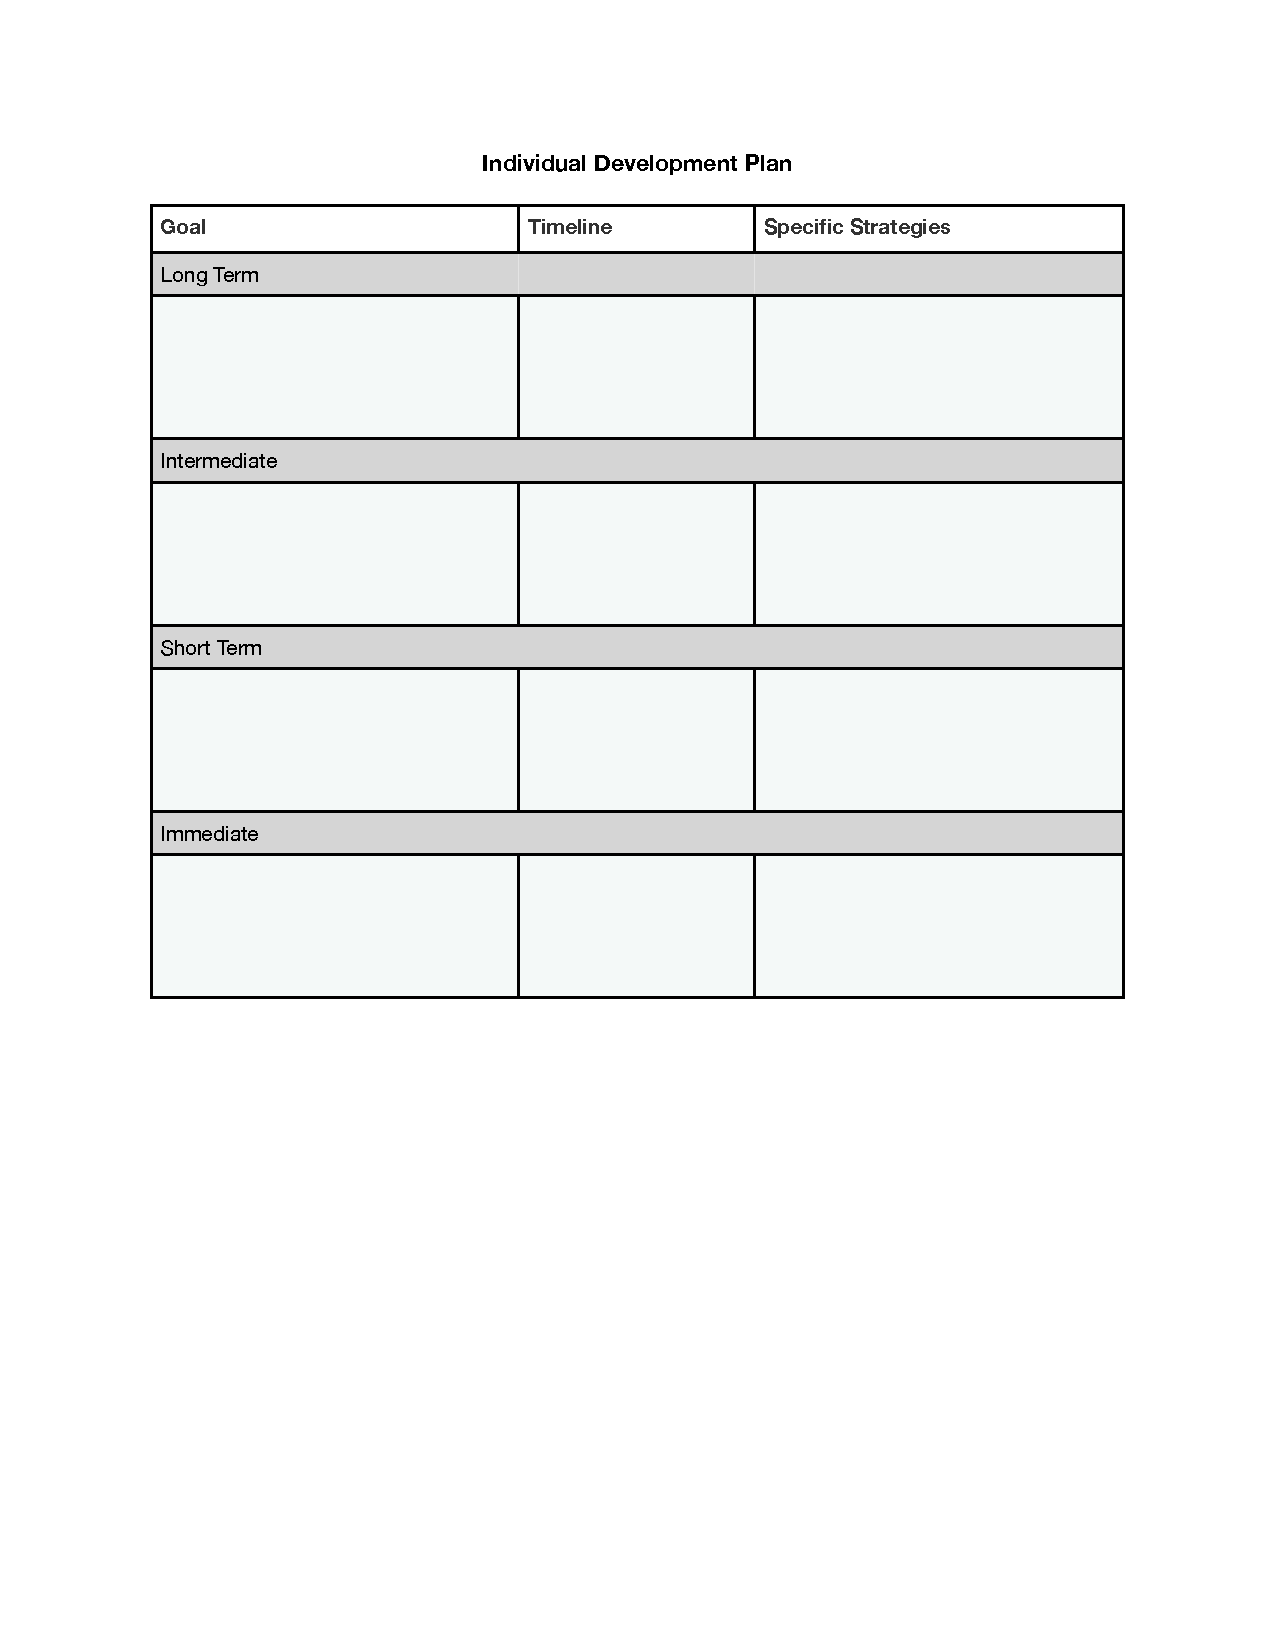
\includegraphics[width=5in]{IDP.pdf}
    \caption{A streamlined version of the Individual Development Plan (adapted from \citet{Bosch}) for use in mentoring PASSAGE students.}
    \label{fig:IDP}
\end{figure}

The second part of the mentoring program is to design and complete a mentoring map. \new{provide the thing!} In order to avoid the pitfalls of relying on one individual to provide all of the mentoring needs of a student, we will develop a network of mentors for each student to ensure that we are meeting the individual mentoring needs for each student.  The mentoring map will include mentors to provide Substantive Feedback, Sponsorship, access to opportunities, Accountability, role models, professional/Academic Development, Emotional Support, Intellectual Community and Safe Space. Sample worksheets for creating mentoring maps are included in the supplemental materials.  Ensuring that the student have identified individuals that can ensure that when they are having a problem, they will be able to find the appropriate person to help. This mentoring map will also help our students identify what areas they still need to find reliable people to fulfill their needs.  As we develop the network of mentors that students can rely on it will also solidify their science community. It will show them that they have a number of dedicated individuals that they can turn to.  This is a document that will be revised on a regular basis especially when it needs to expand to accommodate upcoming transitions so we can begin building the community before the students are there \citep{NAP25568}. 


\subsection{Faculty Mentoring Training}\label{sect:facultytraining}

\reword{consolidate} The PIs will facilitate a mentor training that will ensure that all mentors in the program will be aware of the research based methods of mentoring that have been shown to be effective.  One of the findings of the recent student by the National Academies is that mentoring needs to be intentional.  This requires that our mentors be thinking about a deliberate plan for how to effectively mentor their students and the mentoring training workshop will provide the opportunity for discussion amount mentors and require them to articulate their mentoring styles and goals. This will attempt to bring most mentors on board to providing a thoughtful and deliberate approach to mentoring.  In addition, in these training sessions will include instruction how to create, evaluate and improve the students IDP and mentoring map. These proven tools will provide a structure for the mentors to implement their own mentoring approaches.   


 In order to ensure that our students are receiving quality mentoring experience we will provide a mentor training workshop before the start of each cohort year.  In addition, an end of year reflection meeting will also be held at the end of each year to self assess the effectiveness of policies and activities implemented each year.

Before the start of the year, faculty interested in mentoring S-STEM students will be required to participate in a two hour faculty mentoring workshop.  During the workshop we will cover several main topics.  The first will be an overview of the program and an overview of the students enrolled in the cohort.  It is important that the faculty are aware of the challenges that are facing the students that they have agreed to mentor.  We will highlight some guidelines of sensitivity training and sexual harassment training provided by the  QCC diversity office, to ensure that each mentor is aware of the policies and procedures surrounding appropriate behavior and reporting guidelines.  After the overview of policies procedures and general guidelines for the program, we will describe specific mentoring strategies that have been shown to be effective. We will discuss the creation and maintenance of both mentoring maps and an independent development plan for undergraduates.  Detailed instructions will be provided to the mentors regarding the creation of these documents.  Regular updates of both documents will be required from the mentors.  All of the instructions and strategies for maintaining these documents will be detailed during the mentor training workshops.   There will also be a portion of the mentor training for mentors to share things that worked and things that did not from previous mentoring experiences.  In preparation for the last portion of the workshop each faculty mentor will be asked to complete a quick survey that identifies how many students they can support, a brief description of their project and to identify one thing that worked for them when mentoring and one thing that they tried but was unsuccessful. 

The end of year meeting will be a time to touch base with each of the mentors and get some information about how the year went.  We will conduct informal interviews with each of the mentors regarding their mentoring experience and their perceived experience of the student.  This feedback will then be compared to a student response to ensure that the experience was perceived similarly by both parties in the relationship.  Where conflicts are identified the PIs can intervene and attempt to improve the relationship.




\subsection{Peer Mentoring}

Alongside faculty mentoring, we will set up a peer-mentoring structure.  Each student in an incoming cohort (except the first) will receive a ``buddy'' from the year ahead of them.  This setup will encourage inter-cohort community building, and allow for the sharing of student resources like course advice, tutoring, and  information about transferring, as well as the creation of study groups.  Once students begin transferring to other colleges, we will forge connections between different cohorts who go to the same school.  This network will ease the difficulty in transitioning to a new school with new challenges.  

\subsection{Building a Community of Researchers}

Students will do one summer of research at QCC, but during subsequent summers they will be encouraged to apply for external REUs, internships, or industry experiences.  These experiences will build their networks, teach them new skills, and  increase their experience and exposure to their chosen STEM subfield.  

We will encourage students and faculty to participate in local scientific conferences, such as the Astronomical Society of New York (ASNY) or American Association of Physics Teachers (AAPT) or the Conference of Undergraduate Women in Physics (CUWiP).  Presenting results and meeting scholars from other institutions is a great way to inspire students and motivate them toward academic excellence.  S-STEM scholars will also be required to present their research at QCC Undergraduate Research Day, which occurs at the end of the Fall and Spring semesters.

%emphasize community building.  we have a lot of this required stuff in other sections, so it doesn't need its own section here necessarily, but we should make sure we cover all the bases.


\subsection{Community-Building}
The social aspect of academia is often how the most fruitful relationships between colleagues begin.  We don't want to neglect this aspect so we are proposing regular social experiences for the students enrolled in the program.  These will be both on campus activities such as games, lunches and informal gathers as well as off campus experiences such as going to local museums (e.g. Natural History Museum) and working scientific labs (e.g. Brookhaven) QCC faculty and staff have connections at many institutions in the greater New York area that would make facilitating these outings easier.  This will facilitate in solidifying the cohort structure for the students.  We want to create activities that bond each cohort of students and allow them to learn from the   (also Vassar, Bell Labs)


\section{Expected Outcomes}
Our goal is to retain 75\% of students in STEM fields, including 50\% in physics/astronomy.  Such a success rate would substantially increase the number of physics majors graduating from QCC (currently zero) as well as the overall number of community college students who remain in STEM past the first year.  

There are a plethora of low-income students at QCC who would qualify for our S-STEM scholarships.  The overall student population is \reword{XX,XXX}, and \reword{XX}\% of these are low-income.  However, there are only \reword{xx} students interested in STEM fields, according to the Office of \reword{Blah}.  This is still a large enough number that we do not expect any problems recruiting enough students.  

Year-to-year retention rates for low-income students in STEM fields are low, but with the support we will provide with our program, the rates are likely to increase.  If students do leave the physics/astronomy program, they may remain in another STEM field, such as computer science or engineering.  Overall, out of the 28 students we propose to support here, we hope that all will graduate with an A.S. degree in Physics from QCC.  Eventually, 14 will graduate with a physics or astronomy bachelor's degree, and 7 more will graduate with other STEM degrees.  We expect 1-2 (25\%) of our students to drop out of our program each year, and forfeit their scholarship support from S-STEM.
%For S-STEM eligible disciplines included in the proposal, expected outcomes should include, at a minimum: expected demographics and enrollment for the disciplines that are included in the proposal showing the current number of low-income students that would qualify for the scholarships; expected year to year retention or transfer rates for S-STEM eligible disciplines for the eligible student population that are included in the proposal; expected graduation rates for each of the S-STEM disciplines included in the proposal and/or expected student outcomes documenting students successfully overcoming one or more of an institution’s self-identified attrition points.


%\section{Generation of Knowledge}
%  All projects should advance understanding about the factors and/or activities associated with retention, student success, transfer, academic/career pathways, and degree attainment. Knowledge generation should be based on the information needs of the institution; draw on the research literature on evidence-based practices, student success, and degree attainment; state questions that guide the investigations; and describe how the questions will be answered.



\section{Evaluation}
% S-STEM projects should include a clear and specific project evaluation plan. The evaluation should include formative evaluation for project improvement in the first two years of implementation to allow for any necessary corrective action and summative evaluation to assess and document project outcomes, accomplishments, and lessons learned at the end of the project. Beyond the impact on students, S-STEM projects should collect data to ascertain impact on the departments, disciplines involved, and the institution. Each S-STEM proposal should describe evaluation plans that are clearly aligned with the stated goals of the project. The evaluation design should match the scope of the project.

%The evaluator must be external to the project, but not necessarily to the institution. The evaluator should not be a Co-PI or senior personnel on the project.

%S-STEM projects are required to participate in regular NSF-led data collection activities to follow student progress.

We will perform a quantitative assessment of PASSAGE by tracking the progress of students as they matriculate to four-year institutions and beyond. Specifically, {\bf our goal is for 75\% of participating students to achieve a B.S. in a STEM field, with 50\% in physics and/or astronomy}. We will track the number of students who present their research at the annual QCC Research Day, how many transfer to a STEM major at a four-year college, and how many graduate with a STEM degree.  Along the way, we will also undertake a more qualitative assessment, consisting of surveys and interviews of participating students and faculty mentors.  We shall continually seek to improve the selection process, seminar series, research course, and research experience for all involved.

During Year 2 and Year 5 of our program, we will engage an external evaluator from the CUNY Research Foundation  We have included \$10,000 in the budget per evaluation year, to support our evaluation efforts.  The Year 2 evaluation will serve as a signal that our program is on the right track and enable us to make any course corrections.  The Year 5 evaluation will take all student data into account, and serve as a final and full evaluation of the program.

\section{Dissemination}
%  The results of successful projects will be of potential interest to other faculty, staff, students, other stakeholders, and the community of which the institution is a part, as well as to student services and financial aid professionals and others who operate scholarship programs. The proposal should include a plan to report on the project and its successes and lessons learned to appropriate audiences.

Generation of Knowledge - Could this describe all of those things we know work but apply them to transition instead of retention at one institution?  Yes I guess so.

Once implemented, this model will be ideal for expansion into a department-wide program.  
The PASSAGE program will then become a full QCC-wide, and potentially CUNY-wide, endeavor.

While this proposed model is tailored to QCC, it can easily be exported to other community colleges.  After the first four years, we will create a how-to document and advertise it to other QCC departments as well as nearby colleges, including those in CUNY and SUNY.  We have included funds in our budget to travel to the American Association of Physics Teachers (AAPT) meeting two times, in years 4 and 5, in order to present our results to the broader community.  The proliferation of this program to other departments and institutions is expected to greatly increase the retention of STEM majors during this critical moment in their careers.



%
%% unnecessary!  
%\section{Intellectual Merit}
%
%The students involved in our program will be trained in computer programming, data analysis and visualization, scientific writing, and presentation.  They will not only gain these skills, but also the confidence and ability to innovate in STEM fields.  
%
%\section{Broader Impacts}
%
%Our education plan will involve approximately XX students (XX per year at QCC over YY years) who will conduct scientific research.   The students targeted in our program will mainly be from underrepresented backgrounds; we will select students from the diverse QCC and general CUNY student population who show ``grit'' and the ability to persevere through challenges.  Such students traditionally have lower retention rates in STEM but can be successful when given the proper support.  These students will realize their full potential when they receive these career-building opportunities, making them candidates for future STEM success.  The export of our Physics Pathways program to other colleges will expand the retention of students within other disciplines and at other institutions, further increasing and diversifying our national STEM workforce.   An additional result of our efforts will be the building of a network of equity/inclusion-minded people within the CUNY system and the broader STEM community.
%
%

%This program will expand our national STEM workforce, and its eventual  expansion to other community colleges will multiply that number manyfold.

%\begin{figure}
%\begin{centering}
%\includegraphics[width=4in]{plots/timeline.pdf}
%\caption{Timeline of proposed work. \label{fig:timeline}}
%\vspace{-4mm}
%\end{centering}
%\end{figure}


\vspace{-5mm}
\section{Results of Prior NSF Support}
\vspace{-3mm}
Bellovary is Co-PI on the NSF AAG grant 1812642 "Collaborative Research: Of Mice and Monsters -- Investigating the Growth of Black Holes in Dwarf Galaxies" (9/1/2018 - 8/31/2021)  {\em Intellectual Merit:}  Bellovary serves in a co-advisory role to a Rutgers PhD student (formally advised by Alyson Brooks), whose thesis focuses on black holes in dwarf galaxies in the Romulus simulation.  Our first paper, in which we examine the properties of galaxies which host MBHs which are outliers in the standard scaling relations, was submitted during fall 2019.  {\em Broader Impacts:}  Bellovary is mentoring three community college REU students who are working on observational signatures of wandering black holes in dwarf galaxies.

Riegel is a Co-PI on the NSF REU grant 1359310 "A Community College REU Site for Physics Applications in Astronomy and Biology" (4/23/2014 - 5/31/2021) {\em Intellectual Merit:} Students are engaged in a variety of research projects involving biophysics, space weather, acoustics, particle physics and spectroscopy. {\em Broader Impact:} This program provides community college students authentic research experiences specifically designed for community college students who may not have otherwise had an opportunity to engage in research. 

QCC is part of an existing S-STEM grant in collaboration with SUNY-Binghamton (``Institutional Partnership to Create Successful Student Transition in Smart Energy \& Materials'', Award 1742056).  The authors of this proposal have no involvement with this project.

\newpage
\bibliography{refs}

\end{document}




